\documentclass[10pt,twoside,a4paper]{article}

% Configure these parameters.
% Name and id
\newcommand{\workdate}{05/01/15}
\newcommand{\studentname}{Ben Ramchandani}
\newcommand{\studentid}{bjr39}


\usepackage{graphics}       % Graphics commands
\usepackage{wrapfig}        % Wrapping text around figures
\usepackage{epsfig}         % Embed encapsulated postscript
\usepackage{rotating}       % Extra graphics rotation
\usepackage{longtable}      % Page breaks within tables
\usepackage{supertabular}   % Page breaks within tables
\usepackage{multicol}       % Allows table cells to span cols
\usepackage{multirow}       % Allows table cells to span rows
\usepackage{texnames}       % Macros for common tex names

\usepackage{listings}       % Source code listings
\usepackage{array}          % Array environment
\usepackage{url}            % URL formatting
\usepackage{amsmath}        % American Mathematical Society
\usepackage{amssymb}        % Maths symbols
\usepackage{amsthm}         % Theorems
%\usepackage{mathpartir}     % Proofs and inference rules
\usepackage{verbatim}       % Verbatim blocks
\usepackage{ifthen}         % Conditional processing in tex
\usepackage{xcolor}         % X11 colour names

\usepackage{tikz}
\usetikzlibrary{arrows, automata}
\usepackage{geometry}
\usetikzlibrary{shapes,fit,calc,positioning}

\usepackage{float}

\usepackage{biblatex}
\addbibresource{dissertation.bib}

\usepackage{pgfplots}
\pgfplotsset{compat=1.12}

\usepackage[titletoc,title]{appendix}

\usepackage{placeins}

\usepackage{pdfpages}

\setlength{\oddsidemargin}{-20pt}
\setlength{\evensidemargin}{-20pt}
\setlength{\topmargin}{-65pt}
\setlength{\textwidth}{475pt}
\setlength{\marginparwidth}{100pt}
\setlength{\textheight}{720pt}

\setlength{\parindent}{0em}
\addtolength{\parskip}{1ex}

\usepackage[draft]{changes}


\begin{document}

\author{\studentname}

\date{\workdate}


\textbf{\studentname; \studentid}\\
\textbf{\workdate}\\
\textbf{St Catharine's College}

%%%%%%%%%%%%%%%%%%%%%


\tableofcontents

\listoffigures

\newpage

\section{Introduction}

\subsection{Summary}


\subsection{Aim}

The aim of this project is to allow a user to pay an actor for storing a file on their behalf, without requiring an existing trust relationship between them or a third party.

% No trust.
% Should work for large files.

\subsection{Threat model}

We assume that the Ethereum network is secure, and that the hash function used is not broken*.
The system should be secure against malicious users, who try not to pay,
and against malicious actors who try to get paid without storing the file.

\subsection{Out of scope of this project}

The aim of this project is not to build a distributed file system.
How the actor initially acquires the file, and similarly how the user retrieves it are not considered here.
This project deals only with the incentive to store a file for a fixed time period.
%\subsection{Background}

\subsection{Definitions}

I will explain these as they become relevant, but they are collected here for reference.

\begin{itemize}
\item The \textit{file} refers to the file that is being stored by the system.

\item The \textit{user} is the person uploading the file and creating and funding the contract.

\item An \textit{actor} is someone storing the file on the user's behalf, entitled to the money in the contract.

\item An \textit{attacker} is someone attempting to claim the reward without storing the file.

\item The \textit{contract} is the smart contract on the Ethereum blockchain that responds to proof submissions.

\item  The contract is \textit{active} if it is accepting proof attempts.

\item \textit{Block} refers to blockchain blocks. They are indexed by a number, which is how many blocks have passed since the genesis block.

\item A \textit{Chunk} is a fixed size part of the file.
\end{itemize}

\subsubsection{Variable definitions}

These pertain to the contract, who's definition is parametrised by

\begin{itemize}
\item $T_0$ the block on which the contract is deployed.
\item $N$ the number of blocks the contract should wait after $T_0$ before becoming active.
\item $F$ the file in question. $|F|$ represents is size in bytes.
\item $m$ the number of chunks in the file.
\item $c$ the size, in bytes, of each chunk.
\item $M$, defined as $2^{\lceil \log_2(m) \rceil}$.
\item $X$ the amount of Ether held by the contract.
\end{itemize}

In pseudo code \texttt{||} denotes concatenation of byte arrays.

\section{Preparation}


\subsection{Technical background}

\subsubsection{The Blockchain}

A blockchain is a distributed database that holds its data in an ordered list of records, called blocks.
Each block has, at a minimum, a payload and the hash of the previous block.
In this way, given any block it is possible to use the hashes to trace back a chain of blocks to some initial block.
Provided a secure cryptographic hash function is used, this chain is tamper resistant in that altering any block will break this chain.

\begin{figure}[h]
\begin{tikzpicture}


\coordinate(O1) at (0,0);
\node[below right=0cm of O1,draw, minimum width=3.65cm,minimum height=4cm,fill=white](block1) {$P_i$};
\node[below right=0cm of O1,draw, minimum width=3.65cm,minimum height=1.3cm,fill=white](hash1) {$H_i = h(H_{i-1} || P_{i-1})$};


\coordinate(O1) at (5.25,0);
\node[below right=0cm of O1,draw, minimum width=3.65cm,minimum height=4cm,fill=white](block2) {$P_{i-1}$};
\node[below right=0cm of O1,draw, minimum width=3.65cm,minimum height=1.3cm,fill=white](hash2) {$H_{i-1} = h(H_{i-2} || P_{i-2})$};

\coordinate(O1) at (10.5,0);
\node[below right=0cm of O1,draw, minimum width=3.65cm,minimum height=4cm,fill=white](block3) {$P_{i-2}$};
\node[below right=0cm of O1,draw, minimum width=3.65cm,minimum height=1.3cm,fill=white](hash3) {$H_{i-2} = h(H_{i-3} || P_{i-3})$};

\draw[->, very thick] (hash1) -- (hash2);
\draw[->, very thick] (hash2) -- (hash3);
\draw[->, very thick] (hash3) -- (15.75, -0.65);
\end{tikzpicture}
\caption[A simple blockchain]{A graphical representation of a Blockchain.
Each block consists of a payload $P_i$ and a hash $H_i$ of the previous block.
Here $h$ is the hash function and $||$ denotes concatenation.}
\label{Blockchain}
\end{figure}

\subsubsection{Bitcoin}

The idea for Bitcoin first appeared in 2008 with a paper by the (still unidentified) Satoshi Nakamoto \cite{bitcoin-whitepaper}.
It is based on a continuously growing blockchain, with transactions stored in blocks as the payload.
Creating a new block requires solving a computationally difficult problem, however the solver is rewarded with Bitcoins
in any new blocks they make.
The longest chain is considered the correct one and this allows a distributed consensus to be formed.

The first Bitcoin client was released in 2009, again by Satoshi Nakamoto.
Since then it has been maintained by the community and several other cryptocurrencies have emerged.

% More techincal.

Each user in Bitcoin has a public/private key-pair, with the public key also acting as an address.
Coins may be sent to any address, but spending coins requires the signing of the transaction with the users private key.

Bitcoins are created when new blocks are minted by miners,
in the form of a special transaction awarding Bitcoins to the miner (or any other address of their choosing).

All other transactions consist of a list of input coins, along with proofs of ownership (normally just a digital signature)
and a list of output coins, along with a description of what is required to use them (again normally a digital signature from some address).
The transaction is then signed with the user's private key and broadcast to the network.
Each node in the network verifies that each of the input coins is valid (the unlocking proof is valid
and the coin has not since been spent), that the signature is valid for that address and that the total value of the inputs is at least that of the outputs.
The transaction will then be added to the next block, which each node verifies before beginning work on further blocks.


\subsubsection{Ethereum}


Ethereum is another cryptocurrency, initially propsed in late 2013 \cite{eth-whitepaper}.
it is based on the same ideas as Bitcoin, but extended with a Turing complete language
embedded in the protocol.
There are also several other changes primarily intended to improve performance, however I will not go into those here.
It's base currency is known as Ether.

An address controlled by a blob of code is referred to as a \textit{smart contract}.
The contract analogy holds in the sense that the contract cannot be modified or removed by
its owner or any other party, except in ways defined in the contract itself.
As such, if you put money into a contract, you are bound to its terms.

The contract code is stored on the blockchain and whenever a transaction is sent to its address the code is executed,
and may in turn call other contracts or send Ether to other addresses.
In this way the code becomes part of the block verification process run by all nodes in the network.

To prevent denial of service attacks each step of execution costs money to the transaction sender.
Any transaction intended for a contract should include some amount of `gas', which must be paid for in Ether.
The contract is then run until either it terminates or runs out of gas.

\subsubsection{The EVM}

%Learning a new language counts for something, talk about solidity.

I'll refer to the language used by Ethereum as EVM (Ethereum Virtual Machine) code.
It is a stack based bytecode, with a word size of 256 bits.
Contracts can have multiple entry points and may receive arguments as binary data.

In terms storage contracts have access to:

\begin{itemize}
\item The stack.

For local variables, this is cheap to access (in terms of gas cost).
It does not persist between calls.

\item Memory.

Analogous to the heap, larger structures and arrays can be stored here.
It is slightly more expensive to access.
Memory is not stored on the blockchain, and exists only during the contract execution.

\item Storage.

Permanent storage on the blockchain.
In comparison this is very expensive to access, but allows data to persist between contract invocations.
\end{itemize}

All data sent to or held by a contract is public knowledge as it is shared between all nodes.
As such private data must be stored off chain or encrypted before sending.
The last 256 block hashes are available to the EVM, not including that of the current block (since the block hash depends on the nonce found by the miner, which is not known at block creation).

Full detail on Ethereum and the EVM, including opcodes and associated gas costs can be found in the Ethereum Yellow Paper \cite{eth-yellowpaper}.

\subsection{Solidity}

Solidity is a high-level language that compiles to EVM bytecode.
Originally proposed on August 29th 2014, Solidity is a statically typed object oriented language with JavaScript-like syntax \cite{solidity-proposal}.
It is designed for contract creation and contains several abstractions over EVM code, like dynamically sized arrays, strings and datatypes with sizes smaller than the 256-bit word size.

The language is still in development and their are some limitations not present in EVM bytecode, like the lack of nested dynamic arrays and array slicing \cite{solidity-docs}.

As part of my preparation I learnt Solidity and have used it to write the contract.
The full contract is included in Appendix \ref{app-contract} if you wish to see an example of Solidity code.

\subsubsection{Relevant limitations of Ethereum}

\begin{itemize}
\item No external source of randomness can be used as the computation must be deterministic,
however block hashes may be used for this purpose and cannot be predetermined.

\item All data sent to or held by a contract is public knowledge as it is shared between all nodes.

\item Storing data on the blockchain is expensive (stored by all nodes).
For this reason we cannot simply store the whole file on the blockchain.

\item Sending data to the blockchain is expensive (processed by all nodes).
As such we cannot send the whole file to the blockchain.

\item Extensive computations are expensive.
See section **** %ECC ext.

\item Block hashes are only available for the last 256 blocks.
There are ways to get round this, but it will not be necessary here**.
\end{itemize}


%Advantages:

% Contracts cannot be withdrawn (unless in code)

\subsubsection{Cryptographic hash functions} \label{crypto-hash}

We take the definition used by Merkle \cite{merkle-thesis}.

A cryptographic hash function is a function $h: \{0, 1\}^* \to \{0, 1\}^N$ for some fixed output size $N$.

It has the properties that
\begin{itemize}
\item Given any $x$ it is easy to compute $h(x)$.
\item Given $h(x)$ it is computationally infeasible to find $x$.
\item Given any $x$ it is computationally infeasible to find an $x'$ such that $x \neq x'$ and $h(x) = h(x')$.
\end{itemize}

We take the second property to also cover the case where you are given $x$ and $h(x || y)$ (recall $||$ denotes concatenation), in that it is computationally infeasable to find $y$.
Similarly for $h(y || x)$.

\subsubsection{Merkle trees}

A Merkle tree is a tree-like data structure based on a hash function $h$ in which parent nodes are the hash of their concatenated children.

In our case leaf nodes will be a hash of a chunk of a file.

For example, if we have a file with four chunks $[F_1, F_2, F_3, F_4]$ we can build a Merkle tree by first hashing each chunk to obtain
$[h(F_1), h(F_2), h(F_3), h(F_4)]$, then combining adjacent nodes:
$[h(h(F_1 || h(F_2)), h(h(F_3) || h(F_4))]$.
We use $||$ to denote concatenation.

Finally the {\em root hash} is the root node of the tree, in our case $h(h(h(F_1 || h(F_2)) || h(h(F_3) || h(F_4)))$.
This is more clearly represented in a graphical form.

\begin{figure}[h]
\centering
\begin{tikzpicture}[
	sibling distance=15em,
	every node/.style = {shape=rectangle, rounded corners,
	draw, align=center,
	top color=white, bottom color=white},
	level 2/.style={sibling distance=8em},
	level 3/.style={color=green},
	edge from parent/.style={<-,draw,thick}
]
\node[color=blue]{$M_0 = h(M_1 || M_2)$}
	child { node {$M_1 = h(M_3 || M_4)$}
		child { node {$M_3 = h(F_1)$}
			child { node {$F_1$} } }
		child { node {$M_4 = h(F_2)$}
			child { node {$F_2$} } }
	}
	child { node {$M_2 = h(M_5 || M_6)$}
		child { node {$M_5 = h(F_3)$}
			child { node {$F_3$} } }
		child { node {$M_6 = h(F_4)$}
			child { node {$F_4$} } }
	};
\end{tikzpicture}
\caption[A Merkle Tree]{ A graphical representation of a Merkle tree built from a file $F$ split into 4 chunks $[F_1, F_2, F_3, F_4]$.
Here $||$ represents concatenation.}
\label{Merkle example}
\end{figure}

The file chunks are not considered to be part of the Merkle tree, as such the tree in Figure~\ref{Merkle example} has depth 2.


\subsubsection{RSA}

Let $e$, $p = 2p' + 1$ and $q = 2q' + 1$ be large primes.
Let $N = p \cdot q$.
Find $d$ such that $e d \equiv 1 \mod p'q'$.

Now we have $(m^e)^d \equiv m \mod N$ for all $m \in \mathbb{N}_N$.
Given $e$ and $N$ it is hard to find $d$ unless $p$ and $q$ are known as well.
This therefore forms a public key encryption system.

Notice that $(m_1^e \cdot m_2^e)^d = \left((m_1 \cdot m_2)^e\right)^d \equiv m_1 + m_2 \mod N$, so we can perform multiplication on
encrypted messages $m^e \mod N$. 
That is to say RSA is homomorphic under multiplication.


\subsubsection{Public proofs of retrievability}

A proof of retrievability is proof that one can access a file.
We formalize this using a simplified version of that used by Juels and Kaliski \cite{ecc-por}.

A proof of retrievability is a game between a verifier and an actor.
Intuitively the actor is trying to demonstrate that they hold the file.
An attacker is an actor that tries to trick the verifier without storing the file.



%A slightly more involved example is the verifier sending a key $\kappa$ to the actor.
%They then both run $f_\kappa(F)$ and the verifier compares the results.
%In this case the verifier may precompute $f_\kappa(F)$ and delete the file,
%but still request a verification at a later time.\\

%        --- k --->
%
%  V    <----p ----  A
%
%  emit {1, 0}
%



For our purposes we need a public proof of retrievability, in which the verifier does not have access to the file,
or any other private information.

A PPOR (Public Proof of Retrievability) is described by a three-tuple of the following polynomial-time algorithms.

\begin{itemize}
\item $\texttt{extract}(F) \to \nu$

Takes a file, $F$, and produces a handle, $\nu$, for this file.


\item $\texttt{generate\_proof}(F, \kappa) \to r$

From a file $F$ and value $\kappa$ generate a proof of retrievability $r$.

\item $\texttt{verify}(\nu, \kappa, r) \to \{0, 1\}$

Verify the proof $r$ using $\kappa$ and $\nu$, but without access to the original file $F$.
It must be the case that $\texttt{verify}(\nu, \kappa, \texttt{generate\_proof}(F, \kappa)) = 1$
\end{itemize}

A PPOR scheme $(\texttt{extract}, \texttt{generate\_proof}, \texttt{verify})$ is said to be secure under a monotone function $g: \mathbb{R}_{\geq 0} \to \mathbb{R}_{\geq 0}$ iff
there is no polynomial time function
$\texttt{cheat}(c(F), \kappa) \to r$ for which $\texttt{verify}(\nu, \kappa, \texttt{cheat}(c(F), \kappa))$
is $1$ with more than negligible probability for all sufficiently large $F$,
where $c(F)$ is at most $g(|F|)$ in size.

Under this scheme it is impossible to be secure under any function that grows at least as fast as the identity function on non-negative reals.

A trivial (and trivially correct under all $g \in o(n)$) example would be requiring the actor to send the entire file to the verifier.
In this case $\nu$ and $r$ will simply be $F$ and the verifier will just check that $\nu = r$.

In a contract implementation $\nu$ must be stored on the blockchain
and $r$ must be processed on the blockchain.
Therefore for a scheme to be practical we require that $\nu$ and $r$ are both small in size (e.g. in $o(|F|)$).
In particular the smallest (slowest growing) $g$ for which the scheme is not secure should grow much faster than $\frac{|\nu|}{|F|}$
(an attacker must store much more than any verifier).
The value $\kappa$ will be the blockhash of a block not present when the contract is uploaded.

Clearly the trivial scheme above has $\nu, r \not\in o(|F|)$.

Ones mind might turn to the thought of computing a keyed one way (hash) function ($f_k$) on the file, and using that as the proof,
i.e. $\texttt{generate\_proof}(F, \kappa) = f_\kappa(F)$. To verify we compute $f_\kappa(F)$ and compare.

This fails however.
Note that to verify the file we must either
\begin{itemize}
\item Calculate $f_\kappa(F)$ in \texttt{verify}.

This requires $\nu = F$ (or $\nu$ otherwise contains $F$) which violates $\nu \in o(|F|)$.
\item Be able to construct $f_\kappa(F)$ from $\nu$ and $\kappa$.

However if $\nu \in o(|F|)$, then the attacker can store $\nu$ and do the same reconstruction (note \texttt{extract} does not depend on $\kappa$).
\end{itemize}




\subsubsection{Merkle tree Public Proofs of Retrievability}

Merkle trees provide a way to prove membership of a single chunk of a file in $O(\log(n))$ time and space,
whilst requiring the verifier to have only $O(1)$ information (the root hash).

A proof consists of a chunk of the file, and all the other hashes needed to reach the root hash.

Consider Figure~\ref{Merkle example}.
To produce a proof of membership of chunk $F_3$, for example, we include $F_3$ in full.
We do not need to include $M_5 = h(F_3)$, since this can be calculated from $F_3$.
The aim is to compute the root hash, so we include $M_6$ and $M_1$.\\
A verifier then computes the hash of $M_5 = h(F_3)$, followed by $M_2 = h(M_5 || M_6)$
and finally $M_0 = h(M_1 || M_2)$. They then compare $M_0$ to the known root hash.

\begin{figure}[h]
\centering
\begin{tikzpicture}[
	sibling distance=15em,
	every node/.style = {shape=rectangle, rounded corners,
	draw, align=center,
	top color=white, bottom color=white},
	level 2/.style={sibling distance=8em},
	level 3/.style={color=green},
	edge from parent/.style={<-,draw,thick}
]
\node[color=blue]{$M_0 = h(M_1 || M_2)$}
	child { node[color=red] {$M_1 = h(M_3 || M_4)$}
		child { node {$M_3 = h(F_1)$}
			child { node {$F_1$} } }
		child { node {$M_4 = h(F_2)$}
			child { node {$F_2$} } }
	}
	child { node {$M_2 = h(M_5 || M_6)$}
		child { node {$M_5 = h(F_3)$}
			child { node[color=red] {$F_3$} } }
		child { node[color=red] {$M_6 = h(F_4)$}
			child { node {$F_4$} } }
	};
\end{tikzpicture}
\caption[A Merkle Tree proof of membership]{\em A graphical representation of a Merkle tree built from a file $F$ split into 4 chunks $[F_1, F_2, F_3, F_4]$.
Here $||$ represents concatenation.}
\label{Merkle proof}
\end{figure}


Provided the hash function used satisfies the properties in section~\ref{crypto-hash}
for a cryptographic hash, it is not computationally feasible to fake the proof: the file chunk and the relevant hashes (or the file to reconstruct them) are required.

We can use this proof of membership to create a PPOR by making the chunk required dependent on $\kappa$.

More formally, define
\begin{itemize}
\item $\texttt{extract}(F) = \texttt{root\_hash}(\texttt{Merkle}(F))$


\item $\texttt{generate\_proof}(F, \kappa) =
F[\kappa \mod m] || \text{Merkle tree hashes forming proof}$

Recall $m$ is the number of chunks in the file.
The exact algorithm for proof generation is given later.

\item $\texttt{verify}(\nu, \kappa, r) =
\texttt{extract\_root\_hash}(r) == \nu$

The exact algorithm for proof verification is given later.
\end{itemize}

This scheme gives a constant size to $\nu$ and a logarithmic size for the proof $r$.

This scheme certainly isn't a perfect PPOR, for example an adversary storing only half the file and one hash value has a 50\% chance of being able to generate a valid proof.
However, the chance of being able to successfully generate a proof in polynomial time is not higher than the portion of the file stored.

Formally:

Consider a large file $F$ as a set of equally sized chunks $\{f_1, ..., f_n\}$.
It is the case that
for all subsets $F'$ of $F$
there is no polynomial time function $\texttt{cheat}(c(F), \kappa)$ such that for sufficiently large $F$
\[\mathbb{P}(\texttt{verify}(\nu, \kappa, \texttt{cheat}(c(F), \kappa)) = 1) > \frac{|F'|}{|F|}\]
where $c(F)$ is at most $|F'| + O(\log(|F|))$ in size.\\
That is, the chance of success cannot be greater than the portion of the file that is stored.

This means that it is not more profitable to only store part of a file, provided there is a payout for a valid proof and no consequence for failure.


\subsubsection{RSA Homomorphic encryption proof of retrievability}




\subsubsection{Other proofs of retrievability}

There are a few ways to improve the ratio of file stored to the expected profit.
\begin{itemize}
\item For the scheme described in the previous section, with a payout of $X$ for a valid proof an actor storing a fraction $p$ $\left(=\frac{F'}{F}\right)$ of the file
\[E(\text{profit}) \leq X \cdot p\]

\item Require actors to lock in funds to promise they will provide the proof before hand.
This is an extension and will be discussed later. For a required stake of $L$ we find
\[E(\text{profit}) \leq (X + L) \cdot p - L\]
assuming the stake is returned along with the $X$ payout.

\item A modified Merkle tree algorithm.

A valid proof could be required for two distinct chunks, chosen unpredictably based on $\kappa$.
This makes the expect payout lower when not much of the file is stored, at the cost of doubling the proof length.
\[E(\text{profit}) \leq X \cdot p^2\]

\item Other PPOR protocols exist, one of them is an extension and will be mentioned later.
\end{itemize}



\subsection{Prior work}

\subsubsection{Ethereum Whitepaper}

I first saw the idea for using Ethereum contracts to fund off chain file storage in the Ethereum Whitepaper \cite{eth-whitepaper}.
In this paper I implement and expand on this idea, as well as analyse it's properties.
It also suggests a way to recover the files afterwards, though that is not considered here.

\subsubsection{Proofs of retrievability}

\subsubsection{Filecoin}

Filecoin is a proposal for a Bitcoin-like cryptocurrency and distributed file system in one
that has a proof of retrievability component along with its proof of work function for block mining.
It's whitepaper \cite{filecoin} points to work on compact public proofs of retrievability by Shacham and Waters \cite{compact-por},
however as far as I know Filecoin has never been implemented.

\subsubsection{Swarm, SWEAR and SWINDLE}

Swarm is an overlay for a distributed file system (e.g. IPFS \cite{ipfs}), based on Ethereum.
At the time of writing Swarm is currently in alpha on the Ethereum public test chain \cite{swarm-alpha}.

Swarm has two parts, payment channels to incentivise file exchange and a system similar to the one designed here for incentivising long term storage.

I will describe briefly the long term storage incentive proposed in \cite{swarm-swear-swindle}.

If an owner wishes to pay a node in the Swarm network to ensure that a chunk (Swarm is built around fixed size chunks rather than files)
is stored then the owner pay (via a contract) a node and receives a receipt in return and the storer provides a deposit for the contract.
This receipt contains the hash of the chunk and a validity time and is signed by the storing node.

If the owner (or anyone else who has the receipt) believes that their chunk has not been stored then they go back to the contract with the receipt and a deposit.
This is then a challenge, the deposit must cover the cost of uploading the chunk and the receipt must be valid (checked by the contract).
The storer then has some amount of time to upload the entire chunk to the contract, which can then check that the hash matches that of the receipt.

\begin{itemize}
\item If the challenge is successful (there is no valid chunk uploaded) then the challenger is compensated.
\item Otherwise the storer may recover his funds along with the challenger's deposit that covers the chunk upload cost.
\end{itemize}

If a challenge is not received before the receipt becomes invalid the storer may recover their funds.\\

The approach I will take as some benefits over the one given here under the assumptions I operate under.
%Should consider under challenge is always made for one chunk
\begin{itemize}
\item No interaction is required. The owner does not have to make the challenge themselves. Moreover an incorrect challenge will cost the owner in the Swarm scheme.
\item Merkle tree proofs of retrievability are likely to be shorter, and require less information be held by the client, at least for large files.

Consider the implementation used by Swarm, with a chunk size $C$ (4096 bytes in Swarm), and say the owner wants to ensure an entire file $F$ of size $|F|$.
There will be $\frac{|F|}{C}$ chunks and the owner must therefore store $\frac{|F|}{C}$ receipts.
The chunk hash and signature will both be 32 bytes in size (the hashing functions and Elliptic curve cryptography verification function available to the EVM uses 256 bit keys).
The owner must store at least $64 \cdot \frac{|F|}{C}$ bytes. The proof for any given chunk is $C$ bytes, we assume the owner requests a proof for one random chunk.

In comparison, in a Merkle tree scheme the owner stores nothing and the proof size is $C + 32 \cdot \log_2(\frac{|F|}{C})$.
This encourages a chunk size of around 64 bytes. For a 1MB file the proof size is then 512 bytes.
Choosing to make the proof size equal in the Swarm scheme (so $C = 512$ bytes) we find the owner must store $64 \cdot \frac{1 \text{MB}}{512 \text{bytes}} = 131072$ bytes,
or about 13\% of the original file size. This can be reduced by increasing the chunk size, in exchange for higher transaction fees when a challenge is made.
\end{itemize}

The scheme used by Swarm does have a potentially significant advantage that transaction costs are very low if a challenge is never made.
This makes sense for Swarm as we expect the owner to try and recover the files from the Swarm network before resorting to a challenge as insurance.
As such the higher transaction fees are not a significant issue, though if this litigation procedure becomes common Swarm could benefit from building a 64 byte based Merkle tree
from each chunk when considering receipts and litigation as this would decrease the proof size to 256 bytes.

The scheme used by Swarm is simpler, just a single hash operation.
While this is a good thing, to the EVM the extra complexity is cheaper than the larger transaction size.


\subsection{Why Public POR is required}

I list possible ways one might try and achieve the aim above and why I do something different.

\subsubsection{Trust between user and actor}

Dropbox, for example.
The user trusts that Dropbox will store files, in return for regular payment.

Either the user pays the actor and trusts they will store the file, or the actor stores the file and trusts the user to pay.

\subsubsection{Third party reward holding}

The user could sign a contract promising to pay the actor if they still have the file by a certain date.
In this case the actor is trusting the state and the legal system to ensure they receive payment.

\subsubsection{Put the whole file on the blockchain}

This rapidly becomes prohibitively expensive, so the file must be stored off chain.

\subsubsection{A hash function}

One method would be to have the user store the file themselves and then hash the file under some key,
and ask the actor to do the same.
This however requires trust that the user will initiate the challenge.

This challenge cannot be initiated by a contract, as it requires the contract to know the file.

Likewise storing the hash of the file and requiring the actor upload the whole file for verification will not work as
it is expensive to send data to a contract.

Just hashing the file under some key will not work, as all data in blockchain contracts is public.

\subsection{Design}


\subsubsection{Explanation of design}


The solution therefore must require that a proof of retrievability require the file to construct, but can be verified without access to the file.
It is not necessary that all the file be used in the construction, but it is required that the parts of the file needed cannot be predetermined.

The Merkle tree POR satisfies this.

Merkle tree proofs are only for a single chunk in the file.
It must not be possible to preemptively guess the index of this chunk or the proof could be precalculated and the file discarded.
We use the hash of the block before that the contract becomes active (begins accepting proofs).

\subsubsection{Details of the contract}

The idea is as follows:

The contract is uploaded to the blockchain, containing $X$ ether.
After $N$ blocks it becomes available for submission of proofs.
If a proof is successfully verified the contract pays the sender its $X$ ether.

Contract variables:

\begin{itemize}
\item $T_0$ is the block the contract is created on.
\item $N$ is the number of blocks the contract waits before becoming active.
\item $m$ is the number of chunks in $F$.
\item $H$ is the root hash of the Merkle tree of $F$.
\item $X$ is tge amount of ether the contract holds initially.
\item $\kappa$ is the block hash of block $T_0 + N$.
\item $i$ is the chunk of the file a proof for is required, $i = \kappa \mod m$.
\end{itemize}

The contract should reject a proof submission if:

\begin{itemize}
\item The contract has already paid out.

In the implementation the contract deploys itself upon a successful proof validation,
giving all contained funds to the submitting actor.
In addition to solving this problem, it means the contract need no longer be stored by nodes,
it's creation transaction can be dropped from the blockchain.

\item The block number is $\leq T_0 + N$.
\item The block number is $> T_0 + N + 256$ (can't get block hash).

The current block number is available to the contract so these are simple comparisons.

\item Proof is invalid.

This is discussed below.
\end{itemize}

\subsubsection{Details of the proof algorithm.}

We construct the proof by splitting the file $F$ into chunks of size $c$ bytes.
Let $m$ be the number of chunks in the file, and $M$ be the least power of two greater than or equal to $m$, i.e.
\[M = 2^{\lceil \log_2(m) \rceil}\]

Each chunk is hashed and from this we construct a Merkle tree with $M$ leaf nodes of depth $\log_2(M)$.
If $m < M$ then the extra chunks are considered to be zeroes (these will never be selected for proofs).



The proof key is calculated as $\kappa = \texttt{blockhash}(T_0 + N)$
and the index of the file chunk the proof is for is $i = \kappa \mod m$.

The proof itself is a sequence of bytes containing the selected file chunk $F[i]$ and the other hashes from the Merkle tree required to recover the root hash, e.g


\begin{figure}[h]
\begin{tikzpicture}

\node[draw,minimum width=8cm,minimum height=1cm](chunk) {File chunk $i$; $C$ bytes};
\node[right=0cm of chunk,draw,minimum width=3cm,minimum height=1cm](hash1) {Proof hash 1; 32 bytes};
\node[right=0cm of hash1,draw,minimum width=3cm,minimum height=1cm](hash2) {Proof hash 2; 32 bytes};
\node[right=0cm of hash2,minimum width=2cm,minimum height=1cm](hash2) {\Large\ldots};

\end{tikzpicture}
\caption[Proof structure]{A representation of the structure of a Merkle tree based proof of retrievability.}
\end{figure}


To verify the proof, one first hashes the first $c$ bytes, then concatenates it with the next hash in the proof,
hashes this new value and repeats until the end of the proof.
A valid proof is one that results in the root hash being the final value.
The order in which the hashes are concatenated ($A \,||\, B$ or $B \, || \, A$) depends on $i$, as we mirror a walk up the Merkle tree.
Equivalently it can be thought of do depend on the binary representation of $i$, from least to most significant bit.

The length of the proof will be $C + 32 \log_2(M)$ bytes.
The 32 comes from the 256 bit hash function used.

Pseudo-code for the proof generation and verification is reproduced below.

Have function \texttt{readChunk} that reads the next chunk from the file (and implicitly keeps its position).
\texttt{h} is the hash function, \texttt{||} denotes concatenation and \texttt{array[i, j]} denotes array slicing.

The Java code for these functions may be found in Appendix **.
The Solidity contract which implements the verification algorithm is in Appendix \ref{app-contract}.




\section{Implementation}

%Should this be in evaluation
\subsection{Security considerations}

Security considerations.
Validity of proof mechanism already considered.

Threat model is logical actor wishing to maximize expected payment per byte of storage used.

We assume Ethereum and our hashing algorithm are not compromised.

\subsubsection{Block hash as random number}

\subsubsection{File length is not a multiple of chunk size}

\subsubsection{Number of chunks, $m$, is not a power of two}

If the actor stores the whole file then the payout per chunk is $\frac{X}{m}$.
If the actor were to only store $n < m$ chunks then they must store a strictly positive amount of extra data, $\epsilon$, to be able to reliably construct a valid proof for those $n$ chunks.
The chance that one of these $n$ chunks is chosen is $\frac{n}{m}$.
Therefore the expected payout per chunk is $\frac{n}{m} \cdot \frac{X}{n + \epsilon} = \frac{X}{m + \epsilon'} < \frac{X}{m}$
and the actor will always store the whole file.

This breaks down if the actor cannot store the whole file in which case it can cause some sets of chunks to be more valuble than others.
This edge case is a good reason to implement the lock-in extension (see section \ref{ext-lockin}).

\subsubsection{Block hash availability}

The last 256 block hashes are available, not including that of the current block.
The EVM opcode that retrieves a block hash fails silently if that block is not available, returning 0.
As such the block hash used to generate $i$ must be before the contract becomes active,
and the contract must deactivate 256 blocks after.





\subsection{Proof generator}

% Should be chunk stream...
\subsubsection{BlockStream}

This class is a wrapper around a file that returns fixed size chunks as a byte array.
This means the rest of the code doesn't have to deal with IO.

\subsubsection{Merkle}

My first implementation built the tree in memory, however this can use large amounts of RAM, since the size of the tree grows linearly with the size of the file.

Instead the root hash calculation is done using a recursive function using only $O(\log(|F|))$ space.

We assume we have a function \texttt{readChunk} that returns the next chunk in the file.
The hash function is \texttt{h} and \texttt{||} denotes concatenation.

In pseudo code:

\lstset{
breaklines=true,
basicstyle=\ttfamily\small,
tabsize=4
}
\begin{lstlisting}
fun merkle(depth) {
    if (depth == 0) {
        return h(readChunk());
    } else {
        return h(merkle(depth - 1) || merkle(depth - 1));
    }
}
\end{lstlisting}

The proof generation can then also be expressed as a recursive function.

\begin{lstlisting}
fun proof(depth, i)
    if (depth == 0) {
        readChunk();
    } else {
        M = 2^(depth - 1);
        if (i < M) {
            return proof(depth - 1, i) || merkler(depth - 1);
        } else {
            tmp = merkle(depth - 1);
            return proof(depth - 1, i - M) || tmp;
        }
    }
}
\end{lstlisting}

For testing reasons I also implemented the validation procedure.

\begin{lstlisting}
fun validate(chunkSize, rootHash, proof, i) {
    
    depth = (proof.length - chunkSize) / hashLength;
    hash = h(proof[0, chunkSize]);
    int positionInProof = chunkSize;
    
    for n in 0..(depth-1) {
        otherHash = proof[positionInProof, positionInProof + hashLength];
        if (i % 2 == 0)
            hash = h(hash || otherHash);
        } else {
            hash =h(otherHash || hash);
        }
        i /= 2;
        positionInProof += hashLength;
    }
    return hash == rootHash;
}
\end{lstlisting}

The full Java code for these three functions can be found in Appendix~\ref{app-java}.

\subsection{Changes from the proposal}

\subsubsection{SHA256 $\to$ SHA3 KECCAK}

I'm using a different hash algorithm to SHA256, which I mentioned in the proposal.
This is due to me misunderstanding the documentation when I read it at the time.
Whilst SHA256 is available in EVM code it is in the form of a precompiled contract, not a true opcode,
the intention being to prevent the wasting of opcodes in the language.

As I'll mention later array slicing is not yet implemented in Solidity, so at points I
used an assembly language to improve efficiency.
The SHA256 contract isn't as easily available, so instead I switched to KECCAK-256

SHA3's KECCAK-256 function is available as a true opcode in the EVM.
In my case it's a drop in replacement in the contract, the only downside is having to bring in an external library
to handle it in Java, whilst SHA256 was available from the standard library.


\subsection{Problems encountered during implementation}




\subsection{What I'm not doing}

The DFS, including 


\subsection{Extensions}

\subsubsection{Recovery}

This is an important extension for practical purposes.
The contract should allow the user to recover the funds if no-one submits a valid proof.

The block hash expiry time of 256 blocks gives a natural time-out.
With the current block time of 14 seconds (https://etherscan.io/chart/blocktime)
this is about an hour.

To implement this the contract remembers its owner from its constructor and allows the owner to recover the funds (and destroy the contract) after $T_0 + N + 256$ blocks.

\subsubsection{Lock in} \label{ext-lockin}

The contract can be redesigned such that an actor must lock in a certain amount of funds before some time $T_0 + N'$ (where $N' < N$),
to allow them to claim the reward.

This would give the user confidence that their file is stored, and discourage actors from only storing a subset of the chunks in a file,
or deleting stored data if a better offer is made.

The contract is initially loaded with $X$ Ether.
One actor can send $Y$ Ether to the contract, their address is then stored on the blockchain.
When a proof is submitted the contract will check that the sending address matches, and return $X + Y$ Ether to the actor
on submission of a valid proof.

If the actor does not submit a valid proof while the contract is active, then the full $X + Y$ Ether can be recovered by the user.

It's also possible to take this further, allowing $n$ actors to lock in and all claim rewards.
It is, however, not possible to determine whether the actors are in fact the same person storing the file once, so this is of limited utility.

Simply creating $n$ separate contracts with slightly offset lock-in and activation times might be better, as it means different actors are slightly more
likely to be the first to lock in if there is competition.


\subsubsection{ECC}

It is possible to use techniques based on Elliptic Curve Cryptography (ECC) to create compact proofs of retrievability \cite{ecc-por}.

I've looked into implementing the scheme described in \cite{ecc-por} as an extension, to replace Merkle tree based proofs.
The operations required are considerably more computationally expensive than Merkle trees.
Whilst in theory it should be possible to implement them in Solidity, it is likely that the resulting code would be too expensive to call.
There is currently a project underway to add native code implementations of elliptic curve primitives
as precompiled contracts in the EVM \cite{eip-ecc}.

% What it could do it theory

\subsubsection{Multiple chunk proofs} \label{multi-chunk}

A different way to improve the security of the Merkle tree PPOR is to require proofs of membership for $Y$ chunks in the file.
In this case the chance that an actor as the relevant file chunks storing only $m'$ out of $m$ in total is $\left(\frac{m'}{m}\right)^Y$,
which discourages storing a small portion of a file.
The cost is that the size of the proof $r$ grows linearly with $Y$.

Different chunk numbers for proofs can be extracted from the block hash $\kappa$ by hashing is $Y$ times and taking the value modulo $m$
as the chunk index each time.

\subsubsection{Multiple Merkle trees}

It is possible to alter how the file is split up into chunks. So far we have simply divided the file evenly into parts, however there is no reason we couldn't have taken strips of the file instead.

\begin{figure}[h]
\begin{tikzpicture}

\node[draw, minimum width=2cm,minimum height=3cm,fill=yellow!30](chunk1) {};
\node[right=0cm of chunk1,draw, minimum width=2cm,minimum height=3cm,fill=red!30](chunk2) {};
\node[right=0cm of chunk2,draw, minimum width=2cm,minimum height=3cm,fill=blue!30](chunk3) {};
\node[right=0cm of chunk3,draw, minimum width=2cm,minimum height=3cm,fill=green!30](chunk4) {};

\end{tikzpicture}
\caption[]{Chunks}
\label{file-chunk}
\end{figure}

\begin{figure}[h]
\begin{tikzpicture}

\node[draw, minimum width=0.5cm,minimum height=3cm,fill=yellow!30](chunk1) {};
\node[right=0cm of chunk1,draw, minimum width=0.5cm,minimum height=3cm,fill=red!30](chunk2) {};
\node[right=0cm of chunk2,draw, minimum width=0.5cm,minimum height=3cm,fill=blue!30](chunk3) {};
\node[right=0cm of chunk3,draw, minimum width=0.5cm,minimum height=3cm,fill=green!30](chunk4) {};

\node[right=0cm of chunk4,draw, minimum width=0.5cm,minimum height=3cm,fill=yellow!30](chunk1) {};
\node[right=0cm of chunk1,draw, minimum width=0.5cm,minimum height=3cm,fill=red!30](chunk2) {};
\node[right=0cm of chunk2,draw, minimum width=0.5cm,minimum height=3cm,fill=blue!30](chunk3) {};
\node[right=0cm of chunk3,draw, minimum width=0.5cm,minimum height=3cm,fill=green!30](chunk4) {};

\node[right=0cm of chunk4,draw, minimum width=0.5cm,minimum height=3cm,fill=yellow!30](chunk1) {};
\node[right=0cm of chunk1,draw, minimum width=0.5cm,minimum height=3cm,fill=red!30](chunk2) {};
\node[right=0cm of chunk2,draw, minimum width=0.5cm,minimum height=3cm,fill=blue!30](chunk3) {};
\node[right=0cm of chunk3,draw, minimum width=0.5cm,minimum height=3cm,fill=green!30](chunk4) {};

\node[right=0cm of chunk4,draw, minimum width=0.5cm,minimum height=3cm,fill=yellow!30](chunk1) {};
\node[right=0cm of chunk1,draw, minimum width=0.5cm,minimum height=3cm,fill=red!30](chunk2) {};
\node[right=0cm of chunk2,draw, minimum width=0.5cm,minimum height=3cm,fill=blue!30](chunk3) {};
\node[right=0cm of chunk3,draw, minimum width=0.5cm,minimum height=3cm,fill=green!30](chunk4) {};

\end{tikzpicture}
\caption[A blockchain]{chunk striping}
\label{file-chunk-stripe}
\end{figure}

In this case a chunk consists of several strips, one from each of what would originally been each chunk.

Each different way of splitting up the file will produce a different Merkle tree.
Only one would be required for the proof, selected based on $\kappa$.
This means several root hashes will need to be stored in the contract (so $\nu$ becomes larger),
however the size of the proof doesn't change.

*** I think this means we get an exponent in the number of different trees, same as last time, provided the striping is `orthogonal' in some sense ***

This approach would make contract generation significantly slower
and possibly proof generation as well, especially because the chunks cannot be read sequentially
which would pose problems when considering large files on mechanical drives.


\subsubsection{Erasure codes}

Erasure codes (or Forward Error Correction in Networking) allow a file to be recovered even if part of the data is lost.

%actually do this.



\section{Evaluation}

% Speed of Java program

% Cost (gas) of contract

% Chunk size vs proof size

% Security - Expected profit of cheater under base and extensions

% Number of chunks required for proof.

% Could have multiple Merkle trees with different chunks

\subsection{Gas cost of contract}

As previously explained, calling contracts on Ethereum costs money.
Calling this contract should be as cheap as possible.

\subsection{Time to generate proofs}

The time taken to generate the proof for a file (and to find the root hash for contract generation) should be as low as possible.

It must be possible to generate the proof in the 256 blocks ($\approx 1$ hour)  that the contract is active for,
though in practice this is not an issue, at least for the base contract.

The following graph is for the base contract.
The test was done on my own PC (i3-4330@3.5GHz, 8GB, Samsung 850 Evo SSD).

\subsection{Effect of chunk size} % could be in implementation.

The size of the chunks that the file is split into has an effect on the performance on several aspects of the system.

\subsubsection{Contract and proof generation}

In general, larger chunk sizes improve performance.

\subsubsection{Proof size} \label{chunk-size-proof-size}

Recall that the proof is the chunk concatenated with all the hashes required for a Merkle tree proof of membership.

Let the chunk size be $c$ bytes.
The number of chunks for a file $F$ is therefore $\frac{|F|}{c}$.
The depth of the Merkle tree is $\left\lceil\log_2\left(\frac{|F|}{c}\right)\right\rceil$.

We use a hash algorithm with 256-bit (32 byte) output, so the proof size is
\[|r| = c + 32 \cdot \left\lceil\log_2\left(\frac{|F|}{c}\right)\right\rceil\]

\begin{figure}[h]
\begin{tikzpicture}
  \begin{axis}[ 
    xmin=0, xmax=260,
    xlabel={$c$ (bytes)},
    ylabel={$|r|$ (bytes)},
    domain=0:260,
    samples=522,
    xtick={16, 32, 64, 128, 256},
  ]
    \addplot[color=blue,mark={}]{x + 32 * ceil(log2(1024 / x))}; 
  \end{axis}
\end{tikzpicture}
\label{eval-graph-chunk-size}
\caption[Chunk size graph]{Proof size against chunk size for a 1024 byte file.}
\end{figure}


The size of the proof will always be smallest when $F/c$ is a power of two.
This is because if you increase $c$ slightly in this position then you still need the same number of proof hashes as the Merkle tree must be a power of 2 in size.


If we require $|F|$ to be a power of two then this analysis is simple.
Since $F/c$ is a power of 2, it follows $c$ is a power of two in this case and we find
\[|r| = c + 32\log(c) + 32\log_2(|F|)\]
and so we can simply minimize $c + 32\log(c)$ with respect to $c$, finding that 32 and 64 bytes both give minimums.
Since proof generation benefits from larger chunk sizes 64 bytes is optimal in this case.

If we don't require $|F|$ to be a power of two then this doesn't hold, the full analysis is included in Appendix~\ref{app-chunk-size}

\subsection{Expected profit of attacker}

A reasonable goal is that any actor that doesn't store enough to reconstruct the file should be expected to make a loss.

We make several simplifying assumptions.
\begin{itemize}
\item In what follows we ignore the logarithmic amount of extra data required to build a Merkle tree from a file chunk.
This is generally a reasonable assumption, for example an actor storing one half of the file needs only one extra hash stored to
construct valid proofs for the 50\% of chunks they have stored.

\item We also assume it is impossible to reverse the hash function.
This is effectively true, so can safely be ignored.

\item We ignore transaction fees. One may consider $X$ to be the original Ether placed in the contract minus the transaction fee for a valid proof.
Since contract execution is deterministic (assuming the block the transaction will be included in is known, and no conflicting transactions are included in the interim) it is 
always possible to know whether a proof submission will succeed. It is therefore the case that the transaction cost does nothing to improve the
security of the contract, unlike a password attempt rate limit SSH server, which does help, for example.
\end{itemize}


Let $F'$ be the set of chunks stored by the actor. Write $\frac{|F'|}{|F|}$ for the proportion of the chunks stored.

\subsubsection{Base implementation}

Under these simplifications, in the base system
the expected profit varies directly with the proportion of chunks stored.
\[E(\text{profit}) = X \cdot \frac{|F'|}{|F|}\]

\begin{figure}[H]
\begin{tikzpicture}
  \begin{axis}[ 
    xmin=0, xmax=1,
    ymin=0, ymax=1,
    xlabel={Fraction of file stored $\left(\frac{|F'|}{|F|}\right)$},
    ylabel={Expected profit ($E(\text{profit})$)},
    ytick={0,1},
    yticklabels={0, $X$},
    domain=0:1,
  ]
    \addplot[color=blue,mark={}]{x}; 
  \end{axis}
\end{tikzpicture}

\caption[Expected attacker profit: base implementation]{Expected profit against proportion of chunks stored by actor for the base contract implementation.}
\end{figure}


\subsubsection{Multiple chunk proofs}

See section \ref{multi-chunk} for details.

Some $Y$ number of chunks are requested instead of just one.
\[E(\text{profit}) = X \cdot \left(\frac{|F'|}{|F|}\right)^Y\]

As can be seen in Figure~\ref{eval-graph-multi} this makes it more profitable (in terms of profit per unit of storage)
to store the whole file rather than partial files. The trade-off is that the proof is longer and hence we pay more in transaction costs.

\begin{figure}[H]
\begin{tikzpicture}
  \begin{axis}[ 
    xmin=0, xmax=1,
    ymin=0, ymax=1,
    xlabel={Fraction of file stored $\left(\frac{|F'|}{|F|}\right)$},
    ylabel={Expected profit ($E(\text{profit})$)},
    ytick={0,1},
    yticklabels={0, $X$},
    domain=0:1,
    samples=50,
  ]
    \addplot[smooth,color=blue,mark={}]{x^2}; 
  \end{axis}
\end{tikzpicture}
\label{eval-graph-multi}
\caption[Expected attacker profit: multiple chunk proofs]{Expected profit against proportion of chunks stored by actor for the Multiple chunk proofs extension with $Y = 2$.}
\end{figure}

\subsubsection{Lock-in}

The contract is given $X$ Ether by the owner, and $L$ by the locking in actor.
A validated proof returns the full $X + L$ to the actor.
\[E(\text{profit}) = (X + L) \cdot \frac{|F'|}{|F|} - L\]


\begin{figure}[H]
\begin{tikzpicture}
  \begin{axis}[ 
    xmin=0, xmax=1,
    ymin=-2, ymax=1,
    xlabel={Fraction of file stored $\left(\frac{|F'|}{|F|}\right)$},
    ylabel={Expected profit ($E(\text{profit})$)},
    ytick={-2,0,1},
    yticklabels={$-L$, 0, $X$},
    axis lines=middle,
    x label style={at={(axis description cs:1.02,0.6666666)},anchor=west},
    ylabel near ticks,
    domain=0:1,
  ]
    \addplot[color=blue,mark={}]{3*x - 2}; 
  \end{axis}
\end{tikzpicture}

\caption[Expected attacker profit: lock-in]{Expected profit against proportion of chunks stored by actor for the Lock-in extension with $L = 2X$.}
\end{figure}


\subsubsection{Combining} \label{combine-ext}

Here we combine lock-in with multi-chunk proofs.

\[E(\text{profit}) = (X + L) \cdot \left(\frac{|F'|}{|F|}\right)^Y - L\]

This is a considerable improvement over either extension alone, however it's still possible for an actor to make a  (albeit reduced) profit
whilst not storing the whole file. It is likely the file will be encrypted and so this may render the entire file lost.

\begin{figure}[H]
\begin{tikzpicture}
  \begin{axis}[ 
    xmin=0, xmax=1,
    ymin=-2, ymax=1,
    xlabel={Fraction of file stored $\left(\frac{|F'|}{|F|}\right)$},
    ylabel={Expected profit ($E(\text{profit})$)},
    ytick={-2,0.0,1},
    yticklabels={$-L$, 0, $X$},
    axis lines=middle,
    x label style={at={(axis description cs:1.02,0.6666666)},anchor=west},
    ylabel near ticks,
    domain=0:1,
    samples=50,
  ]
    \addplot[smooth,color=blue,mark={}]{3*x^2 - 2}; 
  \end{axis}
\end{tikzpicture}

\caption[Expected attacker profit: multiple chunk proofs and lock-in]{Expected profit against proportion of chunks stored by actor with both the Lock-in extension and multiple chunk proofs with $L = 2X$ and $Y = 2$.}
\end{figure}

\subsubsection{Erasure codes}

Adding an Erasure code allows us to recover the file if some chunks are lost.
For example, we could add 25\% to the file size to ensure that the file can be recovered even if 20\% (of the now larger file)
is lost.

Combining this with the technique in \ref{combine-ext} allows us to make it unprofitable to not store the whole file.

\begin{figure}[H]
\begin{tikzpicture}
  \begin{axis}[ 
    xmin=0, xmax=1,
    ymin=-2, ymax=1,
    xlabel={Fraction of file stored $\left(\frac{|F'|}{|F|}\right)$},
    ylabel={Expected profit ($E(\text{profit})$)},
    ytick={-2,0,1},
    yticklabels={$-L$, 0, $X$},
    axis lines=middle,
    x label style={at={(axis description cs:1.02,0.6666666)},anchor=west},
    ylabel near ticks,
    domain=0:1,
    samples=50,
  ]
    \addplot[smooth,color=blue,mark={}]{3*x^2 - 2}; 
    \addplot[color=red,mark=none] coordinates {(0.8, -2) (0.8, 1)};
  \end{axis}
\end{tikzpicture}

\caption[Expected attacker profit: erasure code]{Expected profit against proportion of chunks stored by actor with both the Lock-in extension and multiple chunk proofs with $L = 2X$ and $Y = 2$.
The red line represents the proportion (80\%) of the chunks required to fully reconstruct the original file.}
\end{figure}

\subsubsection{ECC}

\section{Conclusion}

%Worth getting better security - probably not, still have to get file back.

\printbibliography

% If multiple contracts wanted, simply encrypt file with different keys.

\begin{appendices}

\section{Proposal}

\includepdf[pages=-]{proposal.pdf}

\section{Contract code} \label{app-contract}

\section{Java proof generation} \label{app-java}

\section{Optimal chunk length} \label{app-chunk-size}

Recall section~\ref{chunk-size-proof-size}.
The size of the proof is:
\[|r| = c + 32 \cdot \left\lceil\log_2\left(\frac{|F|}{c}\right)\right\rceil\]
which can only be minimal when $\frac{|F|}{c}$ is a power of 2.

We have $\frac{|F|}{c} = 2^n$ for some $n \in \mathbb{N}$, so we re-express $|r|$ in terms of $n$.
\[|r| = \frac{|F|}{2^n} + 32 n\]

We attempt to find the minimum, letting $n$ be in $\mathbb{R}$ for now.
\begin{align*}
\frac{d |r|}{d n} = 0 &\implies 32 - \ln(2) \cdot |F| \cdot 2^{-n} = 0\\
&\implies n = \log_2(|F|) - 5 + \log_2(\ln(2))
\end{align*}

An algorithm for computing the optimal chunk size follows from this
\begin{enumerate}
\item Compute the two natural numbers $n_1, n_2$ closest to $\log_2(|F|) - 5 + \log_2(\ln(2))$.
\item Let $c_i = \left\lceil \frac{|F|}{2^{n_i}}\right\rceil$.
\item Take $j \in \{1, 2\}$ such that $c_j + 32 \cdot \log\left(\frac{|F|}{c_j}\right)$ is minimized.
\item $c = c_j$.
\end{enumerate}
\end{appendices}
\end{document}
